\documentclass{thesis-ekf}

\usepackage[T1]{fontenc}
\PassOptionsToPackage{defaults=hu-min}{magyar.ldf}

\usepackage[magyar]{babel}
\footnotestyle{rule=fourth}

\usepackage{paralist}
\usepackage{colortbl}
\usepackage{xcolor}

\usepackage{amsmath}
\usepackage{mathtools}
\usepackage{amssymb}
\usepackage{amsthm}
\usepackage{amsfonts}

\theoremstyle{definition}
\newtheorem{definicio}{Definíció}[chapter]

\DeclareMathOperator{\arctg}{arctg}

\usepackage{listings}

\begin{document}

    \title{Jókai Mór neoabszolutizmus-modellje\\Az új földesúr című regénye alapján}
    \author{Limbek Zsófia}
    \date{2014}
    \institute{Közép-Európa szakirány}
    \logo{
\includegraphics[width=8cm]{mcc_logo-kek}}
    \city{Budapest}
    \supervisor{Csunderlik Péter}

    \maketitle

    \tableofcontents

    \chapter{A modell összetevői}\label{ch:a-modell-osszetevoi}

    \section{A változók és kapcsolatuk}\label{sec:a-valtozok-es-kapcsolatuk}

    Meglátásom szerint egy történelmi regénnyel leírt modell alkotóelemei három csoportba sorolhatók:
        események, személyek és világnézetek (vagy morál, erkölcs, értékrend, ahogy tetszik).
    E három csoport egymáshoz való viszonya meghatározza az egész regényt.
    Az események kategóriája egyértelmű.
    A személyekhez az egyes szereplők céljait, motivációit, és ezekre irányuló döntéseit sorolom,
        míg értékrendjük egy-egy külön változót alkot.

    \begin{figure}[th]
        \centering
        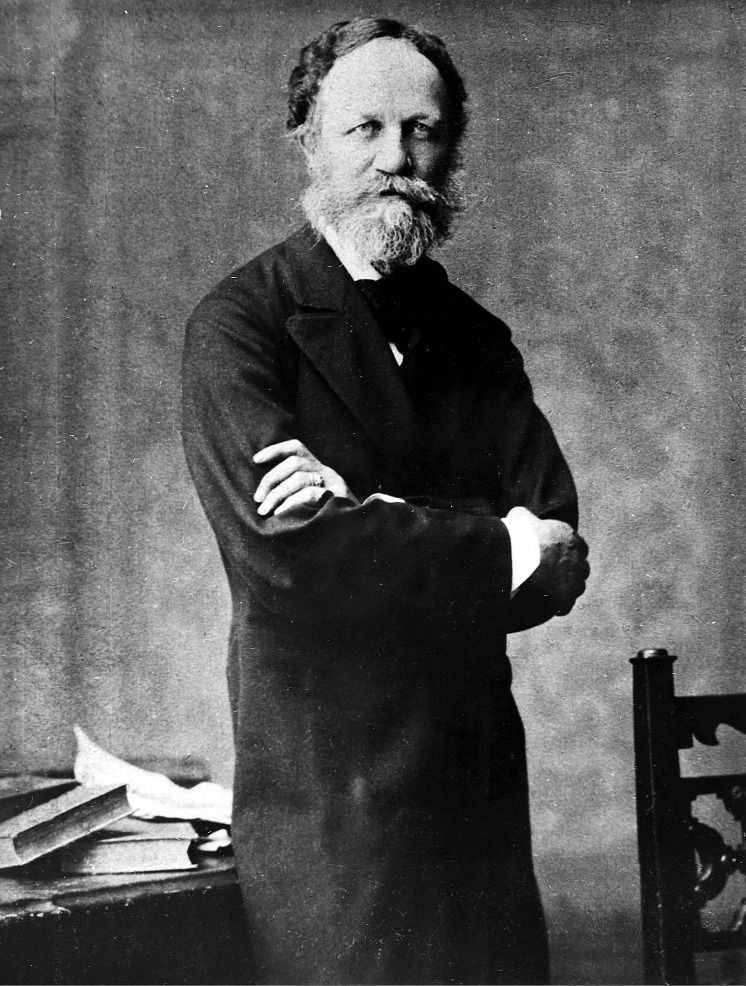
\includegraphics[width=5cm]{jokai-mor}
        \caption{Jókai Mór}
    \end{figure}

    Jókai rendszerint rögzíti az erkölcsi kategóriába tartozó változókat:
        regényeire nem jellemző a jellemfejlődés ábrázolása, a szereplők ebből a szempontból statikusak.
    Határozottan elkülönülnek a ,,jó'' és a ,,rossz'' személyiségek (ha van is köztes kategória, abba csak néhány
        jelentéktelenebb szereplő tartozik)\footnote{Ebben a dolgozatban meghatároztam egy köztes kategóriát,
        amelyet a ,,szerencsétlenek'' csoportjának neveztem el}.
    Az, hogy egy szereplő ezek közül melyikbe tartozik, meghatározza, hogy céljai eléréséhez milyen eszközöket használ fel.

    A személyek és események viszonya már regényenként különbözik.
    Például A kőszívű ember fiaiban és a Török világ Magyarországon-ban az események ,,erősebbek'' a szereplőknél:
        bár a főszereplők mindkét esetben viszonylag nagy hatalommal, befolyással rendelkeznek, mégis nekik kell az
        eseményekhez (pl.~felülről érkező politikai döntés, egy csata vagy háború kimenetele) alkalmazkodniuk.
    Az események itt kívülről adott, exogén változók, míg a személyek cselekedetei
        (természetesen a hozzájuk tartozó erkölcsi jellemzőknek megfelelően) reagálnak azokra, tehát endogének.
    Az új földesúrban ez éppen fordítva van, itt a személyek irányítják az eseményeket.
    Ez alól persze kivétel a kiindulási állapot (a kiépült neoabszolutizmus), de a regény meghatározó történéseire
        (az új szomszéd megjelenése, Aladár kiszabadulása, még az árvíz is ide tartozik) igaz,
        hogy azokat a szereplők akarata és tettei idézték elő.
    Itt tehát a szereplők adottak kívülről, és az eseményeket kapjuk meg a modellből.

    Egy modellt nem csak a változók alkotnak, hanem az azokat összekapcsoló összefüggések is.
    Az új földesúr esetében, hogy az összefüggéseket megtaláljuk, azt kell megnézni, hogy bizonyos szereplők
        találkozásából milyen események következnek.
    Például lehet az egy összefüggés, hogy ahol két jó találkozik, ott valami jó fog történni;
        vagy az, hogy ha egy jó és egy rossz kerül kapcsolatba, akkor a rossz végül alulmarad.
    (Ez két végletesen leegyszerűsített példa, csak a szemléltetés kedvéért hoztam fel őket.)
    Az új földesúr modelljének összefüggéseit a változók leírása után -- \aref{ch:a-modell-osszefuggesei}.~fejezetben,
        \apageref{ch:a-modell-osszefuggesei}.~oldalon kezdődően -- vizsgálom.

    A modell változóinak részletezését a személyekkel kezdem, értékrendjük szerint csoportosítva őket.


    \section{Az új földesúr szereplői}\label{sec:az-uj-foldesur-szereploi}

    A regény szereplői egyrészt jók vagy rosszak, illetve szükségét láttam egy köztes kategóriának is.
    Másrészt el lehet különíteni a szereplőket aszerint is, hogy osztrákok vagy magyarok\footnote{Ez a csoportosítás
        nem teljesen pontos, de szemléletes;~Ankerschmidt lovag nagyrészt cseh származású házanépét az osztrákokhoz sorolom.}.
    Nem meglepő módon a magyarok általában jók, és az osztrákok általában rosszak, de vannak kivételek\footnote{
        A kivételek a regény végére feloldódnak. Természetesen nem a jók válnak rosszakká, vagy fordítva,
        hanem a jó osztrákok (pl.~Ankerschmidt és Eliz) magyarrá válnak, míg a rossz magyarok (pl.~Pajtayné) elosztrákosodnak.}.

    A szereplőkről részletesebb leírás található a függelékben (\ref{ch:fuggelek}.~fejezet),
        ebben a pontban csak felsorolom őket, mint a modell változóit.

    \subsection{,,Jó'' szereplők}

    A jók idealizált karakterek.
    Esetleg furcsa szokásuk, bogaruk lehet, de azok kezelhetők, megszokhatók, más rossz tulajdonáguk pedig nincs.
    Céljaik érthetőek és befogadhatóak, elérésükért tisztességesen küzdenek -- ez a tisztesség időnként megengedi
        a törvények áthágását, máskor viszont törvényben megengedett dolgot tilt.

    A következők tartoznak ide:

    \begin{compactitem}
        \item Garanvölgyi Ádám
        \item Kampós uram
        \item Ankerschmidt lovag
        \item Eliz (később Erzsike)
        \item Garanvölgyi Aladár
    \end{compactitem}

    \subsection{,,Rossz'' szereplők}

    A rossz karakterek sokkal kevésbé kidolgozottak, mint a jók.
    Szerepük kimerül abban, hogy kihívást állítanak a jók elé, illetve időnként megnevettetnek minket.
    A személyiségükről csak annyi derül ki, amennyi e funkciók betöltéséhez szükséges.

    Az új földesúrban feltűnő rossz karakterek:

    \begin{itemize}[\textbullet]
        \item Dr.~Grisák
        \begin{itemize}
            \item osztrák
            \item ügyvéd
            \begin{itemize}
                \item \emph{doctor iuris}
            \end{itemize}
        \end{itemize}
        \item Straff Péter
        \item \begin{itemize}
            \item osztrák
            \item titkosrendőr
            \begin{itemize}
                \item \emph{cabinet noir}
            \end{itemize}
        \end{itemize}
        \item Pajtayné (Corinna)
        \begin{itemize}
            \item magyar
            \item nemesasszony
            \begin{itemize}
                \item \emph{özvegy}
            \end{itemize}
        \end{itemize}
        \item Bräuhäusel úr
        \begin{itemize}
            \item osztrák
            \item hivatalnok
        \end{itemize}
        \item Mikucsek úr
        \begin{itemize}
            \item osztrák
            \item mérnök?
            \begin{itemize}
                \item konkrétan nem derül ki
            \end{itemize}
        \end{itemize}
    \end{itemize}

    \subsection{,,A szerencsétlenek''}

    Ebbe a kategóriába azokat sorolom, akik ugyan nem rosszak vagy rosszindulatúak, de nem is szimpatikusak,
        és nem jönnek rá időben, hogy rosszul döntöttek.
    Ezek a szereplők önmagukban jelentéktelenek, az a legfontosabb funkciójuk, hogy alanyul szolgálnak
        a jók és a rosszak cselekedeteihez, viszonyának bemutatásához.

    Ebbe a csoportba a következőket soroltam:

    \begin{compactitem}
        \item Hermine
        \item Missz Natalie
        \item Maxenpfutsch Vendelin
    \end{compactitem}


    \section{A regény eseményei}\label{sec:a-regeny-esemenyei}

    Az eseményeket tekintem tehát endogén változóknak, ezek azok, amelyek kiszámításához szükségünk van
        a modell összefüggéseire és az eddig ismertetett exogén változókra.
    Az eseményeket csoportokba (cselekményszálakba) rendezem aszerint, hogy mely szereplők befolyásolják őket legerősebben.
    A regény cselekményének részletes leírása a függelékben található, itt csak felsorolom a fontosabb eseményeket.

    Amikor Garanvölgyit írok, az mindig Garanvölgyi Ádámot jelöli, Garanvölgyi Aladárt csak Aladárnak nevezem.

    \subsection{A Garanvölgyi-Ankerschmidt szál}

    \begin{compactitem}
        \item Vita a régi kastélyról
        \item Eliz levele Garanvölgyinek
        \item A yorkshire-i disznók ellopása és a betakarítás Ankerschmidtéknél
        \item Ankerschmidt, Garanvölgyi tudta nélkül, Aladár szabadulásán kezd el ügyködni
        \item A két öregúr között mély barátság alakul ki
        \item Garanvölgyi és Ankerschmidt ,,bajtársak'' lesznek a politika színterén
    \end{compactitem}

    \subsection{A Straff Péter körüli események}

    \begin{compactitem}
        \item Straff Garanvölgyiéknél (mint ál-Petőfi)
        \item Straff Ankerschmidtéknél (mint Bogumil)
        \item Bräuhäusel úr házkutatást tart az ócska kastélyban
        \item Hermine megszöktetése
        \item Straff túlfeszíti az ,,arkhimédeszi csavar''-t
        \item Straff összekeveri Pajtayné leveleit
    \end{compactitem}

    \subsection{Pajtayné játszmái}

    \begin{compactitem}
        \item Pajtayné viszonya udvarlóival és vőlegényével
        \item Pajtayné sikertelen kísérletet tesz a régi udvarlók visszacsalogatására
    \end{compactitem}

    \subsection{Aladár cselekményszála}

    \begin{compactitem}
        \item Eliz beleszeret Aladárba
        \item Ankerschmidt meglátogatja Aladárt a börtönben
        \item Aladár találkozása nagybátyjával, Ankerschmidttel és Pajtaynével
        \item Ankerschmidt és Aladár útja a gátakról hazafelé
        \item Erzsike és Aladár egymásba szeretnek és összeházasodnak
    \end{compactitem}

    \chapter{A modell összefüggései}\label{ch:a-modell-osszefuggesei}

    Eddig igazából csak azonosítottam a regény szereplőit és eseményeit, a dolgozatom érdemi része most következik.
    Ebben a részben azt vizsgálom, hogy a szereplők tulajdonságaiból (exogén változókból)
        hogyan határozódnak meg az események (endogén változók), azaz hogy milyen szabályok léteznek Jókai modelljében.
    Ezek az összefüggések általánosságokat mondanak ki, a konkrét következmények a konkrét résztvevőktől függnek.
    A modell szabályai olyankor érvényesülnek, amikor több szereplő olyan helyzetbe kerül, hogy a céljaik összefüggnek,
        ezért döntéseik hatással vannak egymásra.
    Ezt én az egyszerűség kedvéért találkozásnak nevezem, de jelentheti egyszerűen csak az érdekeik ,,találkozását'' is
        (akár közösek ezek az érdekek, akár ellentétesek).

    Meglátásom szerint elegendő csak a páronkénti találkozásokat vizsgálni.
    Természetesen vannak események, amik kettőnél több szereplő közreműködésével alakulnak ki,
        de a karakterek egymásra gyakorolt hatása parciális, nem függ össze.

    \begin{equation}\label{eq:g-fuggveny}
        g \colon \mathbb{R} \setminus \left\{ \frac{k\pi}{2} : k \in \mathbb{Z}\right\} \rightarrow \mathbb{R}, \qquad
        g(x) \coloneqq
        \begin{cases}
            \frac{\arctg^2(x + \pi)}{\sin(2x)}, & \text{ha } x \geq \frac{2}{3}, \\
            \cos^4 (5x), & \text{különben.}
        \end{cases}
    \end{equation}

    \section{Két jó karakter találkozása}\label{sec:ket-jo-karakter-talalkozasa}

    Jókai legtöbb regényéhez hasonlóan Az új földesúrban is teljesül a következő szabály.
    \begin{definicio}\label{def:ket-jo}
        Ha két jó szereplő találkozik, akkor abból valami jó dolog következik.
    \end{definicio}
    Egyrészt jó kapcsolat alakul ki köztük (barátok lesznek, vagy éppen egymásba szeretnek),
        másrészt amit együtt csinálnak, az is jól sikerül.

    Jó szereplők között kialakuló barátságra a legfontosabb példa Ankerschmidt és Garanvölgyi,
        de Ankerschmidt jó barátságot alakít ki Kampóssal és Aladárral is.
    Együttműködésük eredménye pl.~a jó helyre épült Ankerschmidt-sírbolt, illetve a víz által beszorított emberek kimentése.
    Az eddigieken kívül kívül Garanvölgyi és Erzsike kapcsolata is ide sorolható.
    Természetesen e szabály alapján fejlődik ki Aladár és Erzsike szerelme.

    Láthatjuk, hogy a két jó szereplő találkozására vonatkozó összefüggés a regény összes jó szereplőjére teljesül
        (akik nem a regény során kötnek barátságot, azok már a történet kezdete előtt is barátok voltak).

    \section{Egy jó és egy rossz karakter találkozása}\label{sec:egy-jo-es-egy-rossz-karakter-talalkozasa}

    Szintén jellegzetes Jókai-összefüggés, a következő állítás, ami Az új földesúrra is jellemző.
    \begin{definicio}\label{def:jo-rossz}
        Egy rossz karakter sok fájdalmat és viszontagságot okozhat egy jónak, de végül saját csapdájába esik, és így a jó kerekedik felül.
    \end{definicio}
    Hogy egy ilyen viszony mennyire jelent komoly kihívást a jó szereplőnek, az a két érintett fél szellemi képességeitől,
        intelligenciájától függ.
    Minél okosabb a rossz karakter, annál nagyobb bajt tud keverni, illetve minél okosabb a jó,
        annál kevésbé érinti rosszul a helyzet.

    Erre a szabályra a legfontosabb példa Grisák és Ankerschmidt, illetve Straff és Ankerschmidt találkozása.
        Grisák nem túl okos, inkább csak ráérez arra, hogy hogyan tudja kihasználni a helyzetét.
    Ennek megfelelően az általa okozott problémák lassan jelentkeznek, és viszonylag könnyen kezelhetőek.
    A történet végére Ankerschmidt rájön, hogy Grisák nem jó ember, akinek így valószínűleg elvész az egyik
        legjobban fizető ügyfele.
    \begin{definicio}\label{def:Straff-Grisak}
        Grisákkal ellentétben azonban Straff kifejezetten okos.
    \end{definicio}
    Ennek megfelelően a tettei következményei is komolyabbak
        (pl.~Hermine halála is hozzá köthető).
    Célját (a meggazdagodást) azonban nem sikerül elérnie, tehát alulmarad.

    További példák az összefüggés teljesülésére Pajtayné és Aladár viszonyának alakulása, Kampós uram és
        Bräuhäusel úr találkozása az öreg kastély átkutatása kapcsán, illetve Mikucsek úr és ,,a nép'' interakciója.
    (Ez utóbbi esetben Mikucsek úr a gátszakítással az ott élőknek okoz óriási károkat, Mikucseket ellenben csak
        egyvalaki öli meg, de a gyilkost a nép képviselőjének tekintem.)

    \section{Két rossz karakter találkozása}

    A rossz szereplők találkozására általánosan igaz, hogy eleinte együtt tudnak működni,
        de végeredményben kölcsönösen akadályozzák egymást céljaik elérésében.
    Lásd \aref{eq:g-fuggveny}.~egyenletet.

    Ez az összefüggés a három fő rossz karakter (Grisák, Straff és Pajtayné) között teljesül.
    Miután Hermine meghal, Grisák elesik egy nagyobb összegtől, Straffnak viszont vissza kell mennie a cabinet noir-ba.
    Pajtayné kiszolgáltatná Straffot Ankerschmidtnek, az viszont cserébe megfosztja Corinnát az udvarlóitól.
    És végül, Corinna játszadozik Grisákkal, de Grisák a történet végén minden együtt töltött percet
        kiszámláz neki ügyvédi konzultációként.

    \section{,,A szerencsétlenek''}

    Az előbb kifejtett három összefüggés alkotja a modell magját.
    Jókai azonban árnyalja a képet (javítja a modell pontosságát) azzal, hogy a se nem jó, se nem rossz karakterekre is
        alkalmaz szabályokat.
    Ezek szerint ha egy ,,szerencsétlen'' egy jóval találkozik, az a két szereplő elidegenedésével végződik,
    mivel a ,,szerencsétlen'' nem hajlandó a valójában fontos dolgokkal foglalkozni, ezért nem érti a jókat.
    Erre ad példát Eliz és missz Natalie, vagy Kampós és Maxenpfutsch viszonya.
    Ha egy ,,szerencsétlen'' egy rossz karakterrel találkozik, akkor viszont a rossz jól,
        míg a ,,szerencsétlen'' rosszul jár.
    Ez történik például Straff és Hermine, illetve Straff és Maxenpfutsch esetében.

    Az alább olyan kódrészletet adok közre, amit ennek a beadandó feladatnak az elkészítéséhez használtam.
    A kód elrendezése megfelel a Python konvencióknak és ajánlásoknak.

    \lstinputlisting[language=Python,numbers=left,frame=trbl,caption={Tördelő script}]{formatter.py}

    \chapter{Függelék}\label{ch:fuggelek}

    \section{A regény szereplői}

    \subsection{,,Jó'' szereplők}

    Ebben a részben azokat a szereplőket sorolom fel, akikre \aref{def:ket-jo}.~definíció vonatkozik.

    \paragraph{Garanvölgyi Ádám}
    A regény főszereplője, a passzív ellenállás megtestesítője Ádám úr.
    A szabadságharc bukása, az új rendszer létrejötte és unokaöccsének elvesztése hatására fásult közönybe süllyedt,
        céljairól lemondott.
    Az iránta tanúsított jóindulat belőle is jóindulatot vált ki, míg a rosszindulat makacsságot és szarkazmust.

    \paragraph{Kampós uram}
    Garanvölgyi kasznárja.
    Kampós Ádám úr ellentéte: aktív ellenálló, tevékeny, sokat beszél, folyton jön-megy.
    Gazdájához feltétlenül lojális és ragaszkodó, az ő érdekeit szolgálja mindenek felett.
    Nem olyan okos, mint a körülötte élő uraságok (pl.
    Straff különösebb nehézség nélkül becsapja), de a saját társadalmi szintjén a legintelligensebbek közé tartozik.
    Kampós gyakorlatilag az ideális jószágigazgató.
    Az osztrákoknak rendre túljár az eszén, és közben remekül szórakozik.

    \paragraph{Ankerschmidt lovag}
    A regény másik főszereplője, nyugalmazott katonatiszt;~osztrák, de mégis jó.
    Értékrendje korrekt és szimpatikus, és emellett nagyon szilárd.
    Jó kapcsolatban van Béccsel, de nem feltétlen kiszolgálója a rendszernek.
    Célja egy modern gazdaság létrehozása és működtetése az új birtokon.
    Hiányossága, hogy nem jó emberismerő, amit pl.
    Straff és Grisák is alaposan kihasznál.
    A regény végére elmagyarosodik.

    \paragraph{Eliz (később Erzsike)}
    Ankerschmidt kisebbik lánya, a másik ,,jó osztrák''.
    Apjához hasonlóan karizmatikus egyéniség, vele ellentétben azonban jó emberismerő.
    Erkölcse teljesen egyezik apjáéval, viselkedése viszont kevésbé merev, nőiessége ebben nyilvánul meg.
    Célja egyrészt a család békéjének fenntartása, mikor erre szükség van, másrészt miután beleszeret Aladárba, az ő boldogulása.
    Mindkettőért kész komoly áldozatot vállalni.
    Eliz karaktere igazi romantikus hősnő, a regény végére még a neve is magyar lesz.

    \paragraph{Garanvölgyi Aladár}
    Garanvölgyi Ádám unokaöccse és fogadott fia.
    A történet elején státusfogoly Kufsteinben, még tíz év hátra van a fogságából.
    Talán még az eddigieknél is erősebben idealizált karakter, ami kapcsolatban lehet azzal, hogy Jókai,
        többi főszereplővel ellentétben, egy konkrét valós személyről mintázta\footnote{
        Jókai Mór (1895): Az új földesúr.~Utóhang.
    }.
    Amíg a helyzete reménytelen, beéri kevéssel, de ahogy javulnak a kilátásai, új célokat tűz ki maga elé,
        és keményen dolgozik értük.
    Mindent tisztességesen csinál, a váratlan helyzeteket is mély nyugalommal kezeli, gyorsan és jól tájékozódik.

    \subsection{,,Rossz'' szereplők}
    A rossz karakterek sokkal kevésbé kidolgozottak, mint a jók.
    Szerepük kimerül abban, hogy kihívást állítanak a jók elé, illetve időnként megnevettetnek minket.
    A személyiségükről csak annyi derül ki, amennyi e funkciók betöltéséhez szükséges.

    \paragraph{Dr.~Grisák}
    A korrupt bürokrata karakterét testesíti meg.
    Csak az motiválja, ha valamiből haszna van, tehát ha pénzre, vagy egy fontos pozícióban levő ember kegyére tesz szert.
    A regényben Ankerschmidten élősködik.
    Nem elég gátlástalan azonban ahhoz, hogy kifejezetten gonosz legyen.

    \paragraph{Straff Péter}
    A regény legördögibb figurája: hazug, tisztességtelen, alattomos és gátlástalan;~kihasznál mindenkit, akit csak tud.
    Neki is egyetlen célja, hogy minél több pénzhez jusson, és ennek érdekében akárkinek keresztbe tesz.
    Egyébként eredetileg a ,,cabinet noir'' munkatársa, azaz ő bontja fel és olvassa el a postára adott, gyanúsnak tűnő leveleket.

    \paragraph{Pajtayné}
    Az öreg Garanvölgyi sógornője és Aladár menyasszonya, elosztrákosodott magyar.
    Legfőbb jellemvonása, hogy szívtelen – udvarlói éppúgy hidegen hagyják, mint egykori hazája sorsa.
    Csak a maga hasznát keresi.
    Egy ideig úgy tűnik, hogy ehhez elég okos, de Straffot például alábecsüli.

    \paragraph{Bräuhäusel úr}
    Kerületi biztos, szintén egy korrupt hivatalnok.
    Butasága a regény egyik humorforrása.

    \paragraph{Mikucsek úr}
    Róla még azt sem tudjuk, hogy milyen hivatala van, de ő is a rendszer élősdije.
    Neki nem a butasága, hanem az ügyefogyottsága van kiemelve.

    \subsection{,,A szerencsétlenek''}

    Ebbe a kategóriába azokat sorolom, akik ugyan nem rosszak vagy rosszindulatúak, de nem is szimpatikusak,
        és nem jönnek rá időben, hogy rosszul döntöttek.
    Ezek a szereplők önmagukban jelentéktelenek, az a legfontosabb funkciójuk, hogy alanyul szolgálnak
        a jók és a rosszak cselekedeteihez, viszonyának alakulásához.

    \paragraph{Hermine}
    Ankerschmidt nagyobbik lánya.
    Keveset tudunk róla, csak azt, hogy lelkiismeretes, nagyon szép, és hogy apjához hasonlóan rossz emberismerő.

    \paragraph{Missz Natalie}
    Az Ankerschmidt-lányok nevelőnője.
    Elizt nem tudja kezelni, mivel vele ellentétben képtelen a felszín mögé látni.
    Korlátolt, fontoskodó nő, akivel Straff és Grisák is kedve szerint játszik.

    \paragraph{Maxenpfutsch Vendelin}
    Ankerschmidt jószágigazgatója.
    Kampóssal ellentétben nem ért eléggé a dolgához, viszont nagyképű.
    Mikor felgyorsulnak körülötte az események, nem tudja követni őket, és mindig abban bízik, akiben nem kéne.

    \section{A regény cselekményszálai}

    A regény cselekményét négy szálra bontottam, az alapján, hogy melyik szereplő gyakorolja a legnagyobb befolyást az eseményekre.
    Egy szálon belül a történések időrendben vannak, de az előzmények sokszor másik cselekményszálban találhatók.
    Emiatt elsőre nehéz lehet rekonstruálni az egész regényt a leírásom alapján, de segítségül elkészítettem
        \aref{subsec:Gantt}.~pontban található Gantt-diagramot, ami szerintem jól szemlélteti a cselekmény menetét.

    \subsection{Ankerschmidt és Garanvölgyi}

    \begin{enumerate}[a)]
        \item\label{itm:bekoltoznek} Ankerschmidt lovag földet vásárolt Pajtaynétól, az öreg Garanvölgyi közvetlen szomszédságában,
            és elkezd felépíteni rajta egy modern gazdaságot.
        A két öregúr először azért kerül kapcsolatba, mert Ankerschmidtnek útjában áll egy régi, lakatlan kastély,
            amit azonban Garanvölgyi nem enged lerombolni.
        A viszonyuk így feszülten indul.
        \item\label{itm:Eliz-levele} A következő ponton Ankerschmidt személyesen viszi Garanvölgyihez Eliz levelét, hogy megtudja, mi áll benne.
        A két szomszéd viszonya megenyhül, de továbbra is távolságtartóak maradnak.
        \item\label{itm:gazdasag} Közben nyomon követhetjük az Ankerschmidt-gazdaság helyzetét.
        A lovag hiába ölt bele sok pénzt, nem minden működik terv szerint az első évben, több dolog miatt is nevetség tárgya lesz.
        Kampós felajánlja a segítségét és a tanácsait Maxenpfutschnak, de az csak a saját kárán tanulja meg, 
            hogy Kampósnak volt igaza.
        A szálnak ez a része a nagyképű tudományoskodást állítja szembe az igazi tudással és talpraesettséggel.
        \item\label{itm:Aladarert} Ankerschmidt tudomást szerez Aladárról, és elkezd ügyködni a szabadulása érdekében.
        Megírat egy folyamodványt dr.~Grisákkal, amit Pajtaynéval, mint Aladár menyasszonyával akar letisztáztatni.
        Pajtayné azonban talál rá ürügyet, hogy ezt visszautasítsa.
        \item\label{itm:sirbolt} Hermine halála után Ankerschmidt támogatást kap Garanvölgyiéktől egyrészt a részvétük kifejezése által,
            másrészt Ádám úr felajánlja neki, hogy arra a dombra építtesse az új családi sírboltot, 
            amelyiken a Garanvölgyi családé is van.
        \item\label{itm:politika} Az árvíz és az eljegyzés után már igazi barátok lesznek.
        Ankerschmidt elkezd magyar földesúrként politizálni, és mikor Garanvölgyi végül feladja a passzív ellenállást 
            és visszatér a közéletbe, Ankerschmidttel egymás oldalán harcolnak a magyar érdekeket képviselve.
    \end{enumerate}
    

    \subsection{Straff Péter ámokfutása}

    \begin{enumerate}[a)]
        \item\label{itm:Petofi} Kampós uram Garanvölgyi birtokán bújtatja Straffot, aki elhitette vele, hogy ő Petőfi Sándor.
        Garanvölgyi azonban átlát a szitán, és Kampós elkergeti Straffot.
        \item\label{itm:Bogumil} Straff ekkor álnevet vált, és különböző hazugságokkal beférkőzik Ankerschmidtékhez, ahol végül zongoratanár lesz.
        Missz Natalie és Hermine odavannak érte, csak Eliz idegenkedik tőle.
        Levelet is ír Garanvölgyinek, amiben figyelmezteti, hogy Straff sok mindenről tud, amiből Ádám úrnak baja lehet.
        \item\label{itm:hazkutatas} Straff később kilesi Kampóst a romos kastélyban, jelentést tesz, és emiatt Bräuhäusel úr vezetésével
            vizsgáló bizottság érkezik, hogy házkutatást tartson.
        Ankerschmidt rögtön rájön, hogy Straff adta fel Garavölgyit, és elkergeti a házától.
        \item\label{itm:Hermine-szokese} Amíg azonban Ankerschmidt Bécsben, illetve Kufsteinben van Aladár ügyében,
            Straff Maxenpfutschot és missz Natalie-t kihasználva megszökteti és elveszi Hermine-t.
        Ankerschmidtet megviseli lányának szökése, és nagy lökést ad neki a magyarosodás felé.
        Magyar módra szakállt növeszt, Elizt pedig Erzsikének kezdi hívni.
        \item\label{itm:nincs-hozomany} A körülmények miatt és dr.~Grisák ráhatására Maxenpfutsch és a missz is összeházasodnak.
        Straff azonban csak a pénzéért vette el Hermine-t, és mikor Ankerschmidt, Straff foglalkozása miatt,
            megtagadja Hermine örökségének kiadását, Straff rosszul kezd bánni a feleségével.
        \item\label{itm:Archimedeszi-csavar} Végül Erzsike elintézi, hogy nővére hazamehessen, de Hermine akkor már nagyon beteg.
        A válás meggyógyíthatná, de Straff mindig több és több pénzt akar a válóper aláírásáért cserébe.
        Végül túl sokáig feszíti a húrt, és Hermine meghal.
        \item\label{itm:cabinet-noir} Straff visszakerül korábbi állásába a cabinet noir-ba, és összekeveri Pajtayné leveleit (ld.~lejjebb).
    \end{enumerate}

    \subsection{Pajtayné játszmái}

    \begin{enumerate}[a)]
        \item\label{itm:Corinna-udvarlok} Pajtayné már az első fejezetben szóba kerül, ugyanis a földek, amiket eladott
            Ankerschmidtnek, valójában az öreg Garanvölgyi birtokához tartoztak.
        Pajtayné dr.~Grisák és az új törvények segítségével sajátította ki és adta el őket.
        Itt megismerjük öt udvarlóját, akiket lenyűgöz azzal, hogy mindig annak mutatja magát,
            akit az adott úriember látni szeretne benne.
        Kiderül az is, hogy Straff Pajtayné megbízásából van Garanvölgyi közelében, abból a célból,
            hogy az öregúrra nézve terhelő dolgokat tudjon meg.
        Pajtayné ezeket készül felhasználni arra, hogy Aladár esetleges korábbi szabadulását megakadályozza,
            mivel a házassági szerződésükkel most Aladár járna jobban.
        (Grisák itt két tűz közé kerül, mert Ankerschmidt és Pajtayné is vele akarja elintéztetni Aladár szabadulását,
            illetve nem szabadulását.)
        \item\label{itm:Corinna-Bfured} Aladár kiszabadulása után Bécsbe költözik, ahol azonban majdnem az egész vagyonát elveszti a tőzsdén.
        Azzal a szándékkal, hogy udvarlóival felfrissítse a kapcsolatot, Balatonfüredre utazik.
        De az udvarlóknak írt levelek Straffnál kötnek ki a cabinet noir-ban, aki az egyikben talál egy saját magát fenyegető célzást.
        Ezért bosszúból összekeveri Pajtayné leveleit, hogy mindegyik ahhoz kerüljön, akiről valami rosszat ír.
        Így Pajtayné egyszerre veszti el az összes udvarlóját.
        Végül éppen Straff felé fordulnak a szándékai, de ennek a szálnak a kimenetelét már nem tudjuk meg.
    \end{enumerate}

    \subsection{Aladár}

    \begin{enumerate}[a)]
        \item\label{itm:Eliz-folyamodvany} A régi kastély átkutatása miatt Eliz meglát egy képet Aladárról,
            és elolvassa Ádám úr Aladárhoz írt leveleit.
        Ennek hatására kérvényt ír Aladár szabadulásáért, de a levél persze megint Ankerschmidt kezébe kerül.
        Abban állapodnak meg, hogy Ankerschmidt kieszközöli Aladár szabadon engedését, de Eliz sosem találkozhat Aladárral,
            nehogy úgy tűnjön, mintha érdekből segített volna neki.
        \item\label{itm:varborton} Ankerschmidt meglátogatja a börtönben Aladárt, és gorombáskodik vele, hogy elterelje magáról a gyanút.
        \item\label{itm:Aladar-hazaer} Aladár, miután kiszabadul, hazamegy a nagybátyjához, és visszaadja a látogatást Ankerschmidtnek.
        Ezután felkeresi Pajtaynét, és felbontja vele a házassági szerződést.
        Mély tiszteletet vált ki dr.~Grisákból csak azzal, hogy nem él vissza a szerződés adta lehetőségeivel.
        \item\label{itm:a-kozos-baj} Mivel birtokait nem kapta vissza, mérnökként dolgozik a Tisza-szabályozásnál.
        Hazaüzen Garanvölgyiék falujába, hogy készüljenek fel az árvízre, mert a gátak nem elég biztosak.
        Itt válik fontossá egy beszélgetés dr.~Grisák és Bräuhäusel úr között még a regény elejéről, amiből kiderül,
            hogy nem az előírásoknak megfelelően építtették a gátat, a pénz egy részét zsebre tették.
        Pont ezt a részt igyekszik most Aladár helyrehozni.
        Ankerschmidt saját szemével akar meggyőződni a helyzetről, de amíg a gáton van, Mikucsek úr, akit valószínűleg
            valaki felbérelt erre, átszakítja a gátat egy feljebbi szakaszon.
        Aladár és Ankerschmidt ezért egy kis csónakon eveznek haza a falujukba, és út közben segítenek egy falunyi embernek
            megmenekülni a víztől.
        Garanvölgyiék hallgattak Aladár üzenetére, de Ankerschmidték nem, és az Ankerschmidt-kastély félig összedől
            az árvíz miatt, mivel hanyagul építették.
        Mire Aladárék hazaérnek, az embereket és az értékeket már átmenekítették Garanvölgyihez, és Ankerschmidték
            be is költöznek hozzájuk.
        \item\label{itm:Aladar-es-Erzsike} Erzsike és Aladár megismerkednek, és Aladár rájön, hogy Erzsike írta az őt kiszabadító folyamodást.
        Itt már nyilvánvaló, hogy egymásba szerettek, de Aladárnak erkölcsi problémája van a helyzettel.
        Viszont mikor Ankerschmidttől megtudja, hogy birtokait visszaszerezheti, már nem áll ellent a vonzalomnak,
            és eljegyzi Erzsikét.
        \item\label{itm:per} Mikucsek urat megölik, amiért átszakította a gátat, Aladár és Ankerschmidt lovag tanúként szerepelnek az ügyben.
\end{enumerate}

    \subsection{A regény cselekményszálainak ábrázolása Gantt-diagramon}\label{subsec:Gantt}

    A táblázat fejlécében található római számok a fejezetek számai, a színezett cellákban található betűjelek az
        adott cselekményszálnak az előző pontban a megfelelő betűvel jelölt részeit jelentik.
    Az V.~fejezetnél lévő halványzöld \ref{itm:a-kozos-baj}) arra a beszélgetésre utal dr.~Grisák és Bräuhäusel úr között,
        aminek akkor még semmi jelentőségét nem látjuk, de a XIV.~fejezetben fontossá válik.

    \vspace*{18pt}

    \hspace*{-2.5cm}
    \setlength\tabcolsep{2.3pt}
    \begin{tabular}{ |l|c|c|c|c|c|c|c|c|c|c|c|c|c|c|c|c|c|c|c|c| }
        \hline
        & \small{I.} & \small{II.} & \small{III.} & \small{IV.} & \small{V.} & \small{VI.} & \small{VII.} & \small{VIII.}
        & \small{IX.} & \small{X.} & \small{XI.} & \small{XII.} & \small{XIII.} & \small{XIV.} & \small{XV.} & \small{XVI.}
        & \small{XVII.} & \small{XVIII.} & \small{XIX.} \\
        \hline
        1. A két öreg & \cellcolor{yellow}\ref{itm:bekoltoznek}) & & & \cellcolor{yellow}\ref{itm:Eliz-levele}) &
        \cellcolor{yellow}\ref{itm:gazdasag}) & \cellcolor{yellow}\ref{itm:Aladarert})
        & & & & & & & \cellcolor{yellow}\ref{itm:sirbolt}) & & & \cellcolor{yellow}\ref{itm:politika}) & & &
        \cellcolor{yellow}\ref{itm:politika}) \\
        \hline
        2. Straff & & \cellcolor{red}\ref{itm:Petofi}) & \cellcolor{red}\ref{itm:Bogumil}) & & & &
        \cellcolor{red}\ref{itm:hazkutatas}) & \cellcolor{red}\ref{itm:Hermine-szokese}) &
        \cellcolor{red}\ref{itm:nincs-hozomany}) & & \cellcolor{red}\ref{itm:Archimedeszi-csavar}) &
        \cellcolor{red}\ref{itm:Archimedeszi-csavar}) & & & & & & \cellcolor{red}\ref{itm:cabinet-noir}) & \\
        \hline
        3. Pajtayné & & & & & & \cellcolor{cyan}\ref{itm:Corinna-udvarlok}) & & & & & & & & & & & &
        \cellcolor{cyan}\ref{itm:Corinna-Bfured}) & \\
        \hline
        4. Aladár & & & & & \cellcolor{lime}\ref{itm:a-kozos-baj}) & & \cellcolor{green}\ref{itm:Eliz-folyamodvany}) & &
        \cellcolor{green}\ref{itm:varborton}) & \cellcolor{green}\ref{itm:Aladar-hazaer}) & & & &
        \cellcolor{green}\ref{itm:a-kozos-baj}) & \cellcolor{green}\ref{itm:Aladar-es-Erzsike}) & & \cellcolor{green}\ref{itm:per}) & &  \\
        \hline
    \end{tabular}
    \hspace*{2.5cm}

    \begin{thebibliography}{}
        \bibitem[Jókai (1895)]{foldesur} Jókai Mór (1895): Az új földesúr. Magyar Elektronikus könyvtár.
            Elérhető: \url{http://mek.oszk.hu/00600/00693/html/index.htm}. Hozzáférés ideje: \emitdate{c}{2014-11-28}.
        \bibitem[Balla (2012)]{kihagytak} Balla István (2012): Arató: Hoffmannt kihagyták. Interjú Arató Lászlóval.~fn.hir24.hu, \emitdate{c}{2012-02-28}
            Elérhető: \url{http://fn.hir24.hu/nagyinterju/2012/02/28/hoffmannt-kihagytak-az-alaptantervbol/}. Hozzáférés ideje: \emitdate{c}{2014-11-28}.
        \bibitem[Imre (2004)]{ven} Imre László (2004): Fried István: Öreg Jókai nem vén Jókai. Tiszatáj, 2004.~szeptember, 55-59.
        \bibitem[Ismeretlen (2014)]{jokai} \url{http://www.literatura.hu/irok/romantik/jokai.htm}. Hozzáférés ideje: \emitdate{c}{2014-11-28}.
        \bibitem[Ismeretlen (2014)]{unalmas} \url{http://www.konyv7.hu/magyar/egyeb-menupontok/blogok/a-szerk-blogja/unalmas-remekmuvek}.
            Hozzáférés ideje: \emitdate{c}{2014-11-28}.
    \end{thebibliography}


\end{document}
